\documentclass[twoside]{book}

% Packages required by doxygen
\usepackage{fixltx2e}
\usepackage{calc}
\usepackage{doxygen}
\usepackage[export]{adjustbox} % also loads graphicx
\usepackage{graphicx}
\usepackage[utf8]{inputenc}
\usepackage{makeidx}
\usepackage{multicol}
\usepackage{multirow}
\PassOptionsToPackage{warn}{textcomp}
\usepackage{textcomp}
\usepackage[nointegrals]{wasysym}
\usepackage[table]{xcolor}

% Font selection
\usepackage[T1]{fontenc}
\usepackage[scaled=.90]{helvet}
\usepackage{courier}
\usepackage{amssymb}
\usepackage{sectsty}
\renewcommand{\familydefault}{\sfdefault}
\allsectionsfont{%
  \fontseries{bc}\selectfont%
  \color{darkgray}%
}
\renewcommand{\DoxyLabelFont}{%
  \fontseries{bc}\selectfont%
  \color{darkgray}%
}
\newcommand{\+}{\discretionary{\mbox{\scriptsize$\hookleftarrow$}}{}{}}

% Page & text layout
\usepackage{geometry}
\geometry{%
  a4paper,%
  top=2.5cm,%
  bottom=2.5cm,%
  left=2.5cm,%
  right=2.5cm%
}
\tolerance=750
\hfuzz=15pt
\hbadness=750
\setlength{\emergencystretch}{15pt}
\setlength{\parindent}{0cm}
\setlength{\parskip}{3ex plus 2ex minus 2ex}
\makeatletter
\renewcommand{\paragraph}{%
  \@startsection{paragraph}{4}{0ex}{-1.0ex}{1.0ex}{%
    \normalfont\normalsize\bfseries\SS@parafont%
  }%
}
\renewcommand{\subparagraph}{%
  \@startsection{subparagraph}{5}{0ex}{-1.0ex}{1.0ex}{%
    \normalfont\normalsize\bfseries\SS@subparafont%
  }%
}
\makeatother

% Headers & footers
\usepackage{fancyhdr}
\pagestyle{fancyplain}
\fancyhead[LE]{\fancyplain{}{\bfseries\thepage}}
\fancyhead[CE]{\fancyplain{}{}}
\fancyhead[RE]{\fancyplain{}{\bfseries\leftmark}}
\fancyhead[LO]{\fancyplain{}{\bfseries\rightmark}}
\fancyhead[CO]{\fancyplain{}{}}
\fancyhead[RO]{\fancyplain{}{\bfseries\thepage}}
\fancyfoot[LE]{\fancyplain{}{}}
\fancyfoot[CE]{\fancyplain{}{}}
\fancyfoot[RE]{\fancyplain{}{\bfseries\scriptsize Generated by Doxygen }}
\fancyfoot[LO]{\fancyplain{}{\bfseries\scriptsize Generated by Doxygen }}
\fancyfoot[CO]{\fancyplain{}{}}
\fancyfoot[RO]{\fancyplain{}{}}
\renewcommand{\footrulewidth}{0.4pt}
\renewcommand{\chaptermark}[1]{%
  \markboth{#1}{}%
}
\renewcommand{\sectionmark}[1]{%
  \markright{\thesection\ #1}%
}

% Indices & bibliography
\usepackage{natbib}
\usepackage[titles]{tocloft}
\setcounter{tocdepth}{3}
\setcounter{secnumdepth}{5}
\makeindex

% Hyperlinks (required, but should be loaded last)
\usepackage{ifpdf}
\ifpdf
  \usepackage[pdftex,pagebackref=true]{hyperref}
\else
  \usepackage[ps2pdf,pagebackref=true]{hyperref}
\fi
\hypersetup{%
  colorlinks=true,%
  linkcolor=blue,%
  citecolor=blue,%
  unicode%
}

% Custom commands
\newcommand{\clearemptydoublepage}{%
  \newpage{\pagestyle{empty}\cleardoublepage}%
}

\usepackage{caption}
\captionsetup{labelsep=space,justification=centering,font={bf},singlelinecheck=off,skip=4pt,position=top}

%===== C O N T E N T S =====

\begin{document}

% Titlepage & ToC
\hypersetup{pageanchor=false,
             bookmarksnumbered=true,
             pdfencoding=unicode
            }
\pagenumbering{alph}
\begin{titlepage}
\vspace*{7cm}
\begin{center}%
{\Large Heislab }\\
\vspace*{1cm}
{\large Generated by Doxygen 1.8.13}\\
\end{center}
\end{titlepage}
\clearemptydoublepage
\pagenumbering{roman}
\tableofcontents
\clearemptydoublepage
\pagenumbering{arabic}
\hypersetup{pageanchor=true}

%--- Begin generated contents ---
\chapter{File Index}
\section{File List}
Here is a list of all documented files with brief descriptions\+:\begin{DoxyCompactList}
\item\contentsline{section}{source/{\bfseries Door\+\_\+logic.\+c} }{\pageref{Door__logic_8c}}{}
\item\contentsline{section}{source/{\bfseries Door\+\_\+logic.\+h} }{\pageref{Door__logic_8h}}{}
\item\contentsline{section}{source/{\bfseries floors.\+c} }{\pageref{floors_8c}}{}
\item\contentsline{section}{source/{\bfseries floors.\+h} }{\pageref{floors_8h}}{}
\item\contentsline{section}{source/\hyperlink{hardware_8h}{hardware.\+h} \\*Driver for the elevator hardware }{\pageref{hardware_8h}}{}
\item\contentsline{section}{source/{\bfseries main.\+c} }{\pageref{main_8c}}{}
\item\contentsline{section}{source/{\bfseries order\+\_\+handler.\+c} }{\pageref{order__handler_8c}}{}
\item\contentsline{section}{source/\hyperlink{order__handler_8h}{order\+\_\+handler.\+h} \\*Functions that record, change or delete orders and lights }{\pageref{order__handler_8h}}{}
\item\contentsline{section}{source/{\bfseries Timer.\+c} }{\pageref{Timer_8c}}{}
\item\contentsline{section}{source/\hyperlink{Timer_8h}{Timer.\+h} }{\pageref{Timer_8h}}{}
\end{DoxyCompactList}

\chapter{File Documentation}
\hypertarget{Door__logic_8h}{}\section{source/\+Door\+\_\+logic.h File Reference}
\label{Door__logic_8h}\index{source/\+Door\+\_\+logic.\+h@{source/\+Door\+\_\+logic.\+h}}


Logic for whenever the door would open.  


This graph shows which files directly or indirectly include this file\+:\nopagebreak
\begin{figure}[H]
\begin{center}
\leavevmode
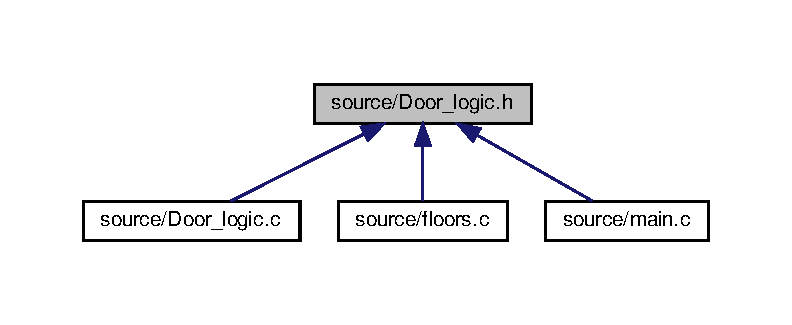
\includegraphics[width=350pt]{Door__logic_8h__dep__incl}
\end{center}
\end{figure}
\subsection*{Functions}
\begin{DoxyCompactItemize}
\item 
void \hyperlink{Door__logic_8h_a2b6685f440423762b93afb3fd14e043d}{door\+\_\+logic} (int $\ast$inside, int $\ast$up, int $\ast$down, int $\ast$next, int current\+\_\+floor, int last\+\_\+direction)
\begin{DoxyCompactList}\small\item\em Uses timer.\+h and stops for 3 seconds when the door would open. As long as {\ttfamily hardware\+\_\+read\+\_\+stop\+\_\+signal} or {\ttfamily hardware\+\_\+read\+\_\+obstruction\+\_\+signal} is active the door will stay open. Door will also stay open for 3 seconds after {\ttfamily hardware\+\_\+read\+\_\+stop\+\_\+signal} goes low. \end{DoxyCompactList}\end{DoxyCompactItemize}


\subsection{Detailed Description}
Logic for whenever the door would open. 



\subsection{Function Documentation}
\mbox{\Hypertarget{Door__logic_8h_a2b6685f440423762b93afb3fd14e043d}\label{Door__logic_8h_a2b6685f440423762b93afb3fd14e043d}} 
\index{Door\+\_\+logic.\+h@{Door\+\_\+logic.\+h}!door\+\_\+logic@{door\+\_\+logic}}
\index{door\+\_\+logic@{door\+\_\+logic}!Door\+\_\+logic.\+h@{Door\+\_\+logic.\+h}}
\subsubsection{\texorpdfstring{door\+\_\+logic()}{door\_logic()}}
{\footnotesize\ttfamily void door\+\_\+logic (\begin{DoxyParamCaption}\item[{int $\ast$}]{inside,  }\item[{int $\ast$}]{up,  }\item[{int $\ast$}]{down,  }\item[{int $\ast$}]{next,  }\item[{int}]{current\+\_\+floor,  }\item[{int}]{last\+\_\+direction }\end{DoxyParamCaption})}



Uses timer.\+h and stops for 3 seconds when the door would open. As long as {\ttfamily hardware\+\_\+read\+\_\+stop\+\_\+signal} or {\ttfamily hardware\+\_\+read\+\_\+obstruction\+\_\+signal} is active the door will stay open. Door will also stay open for 3 seconds after {\ttfamily hardware\+\_\+read\+\_\+stop\+\_\+signal} goes low. 

Opens the doors, then starts the timer. It will remain in the while loop as long as the timer is less than 3 seconds, and it will be reset every time the stop button or obstruction is activated. After 3 seconds it will close the doors, then return from the function.


\begin{DoxyParams}[1]{Parameters}
\mbox{\tt in}  & {\em current\+\_\+floor} & The floor we are currently at\\
\hline
\mbox{\tt in}  & {\em last\+\_\+direction} & The direction the elevator is travelling. 1= up, 2 = down, 0 = stop\\
\hline
\mbox{\tt in,out}  & {\em inside} & The array of the orders from inside the elevator\\
\hline
\mbox{\tt in,out}  & {\em up} & The array of the orders from outside the elevator going up\\
\hline
\mbox{\tt in,out}  & {\em down} & The array of the orders from outside the elevator going down\\
\hline
\mbox{\tt in,out}  & {\em next} & The array that contains the next orders \\
\hline
\end{DoxyParams}


Definition at line 10 of file Door\+\_\+logic.\+c.


\hypertarget{floors_8h}{}\section{source/floors.h File Reference}
\label{floors_8h}\index{source/floors.\+h@{source/floors.\+h}}


function that set the global variables used in almost every function  


This graph shows which files directly or indirectly include this file\+:\nopagebreak
\begin{figure}[H]
\begin{center}
\leavevmode
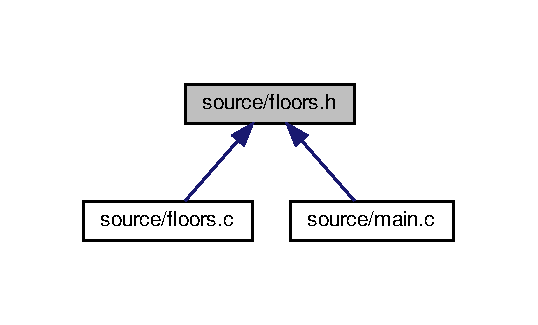
\includegraphics[width=258pt]{floors_8h__dep__incl}
\end{center}
\end{figure}
\subsection*{Enumerations}
\begin{DoxyCompactItemize}
\item 
\mbox{\Hypertarget{floors_8h_a198bc369c49dcd6366ac7554c1fd9d78}\label{floors_8h_a198bc369c49dcd6366ac7554c1fd9d78}} 
enum \hyperlink{floors_8h_a198bc369c49dcd6366ac7554c1fd9d78}{F\+S\+M\+\_\+state} \{ \newline
{\bfseries Init}, 
{\bfseries Stationary\+\_\+f}, 
{\bfseries Stop}, 
{\bfseries Down}, 
\newline
{\bfseries Up}, 
{\bfseries Stationary\+\_\+n}
 \}\begin{DoxyCompactList}\small\item\em The different states used by the F\+SM. \end{DoxyCompactList}
\end{DoxyCompactItemize}
\subsection*{Functions}
\begin{DoxyCompactItemize}
\item 
\mbox{\Hypertarget{floors_8h_a48b4d8842c82a41bdddc846d9e254578}\label{floors_8h_a48b4d8842c82a41bdddc846d9e254578}} 
void \hyperlink{floors_8h_a48b4d8842c82a41bdddc846d9e254578}{read\+\_\+floor} ()
\begin{DoxyCompactList}\small\item\em Changes the global variables above. at\+\_\+floor will be changed to 1 when it is at a floor and 0 when not on a floor. current\+\_\+floor will be changed whenever it is at a floor. \end{DoxyCompactList}\end{DoxyCompactItemize}
\subsection*{Variables}
\begin{DoxyCompactItemize}
\item 
\mbox{\Hypertarget{floors_8h_a53f0cf8d6c7426344a7336af4b06925a}\label{floors_8h_a53f0cf8d6c7426344a7336af4b06925a}} 
int {\bfseries current\+\_\+floor}
\item 
\mbox{\Hypertarget{floors_8h_a068daecb90e86b1e5ec31342937e8ab6}\label{floors_8h_a068daecb90e86b1e5ec31342937e8ab6}} 
\+\_\+\+Bool {\bfseries at\+\_\+floor}
\end{DoxyCompactItemize}


\subsection{Detailed Description}
function that set the global variables used in almost every function 


\hypertarget{hardware_8h}{}\section{source/hardware.h File Reference}
\label{hardware_8h}\index{source/hardware.\+h@{source/hardware.\+h}}


Driver for the elevator hardware.  


This graph shows which files directly or indirectly include this file\+:\nopagebreak
\begin{figure}[H]
\begin{center}
\leavevmode
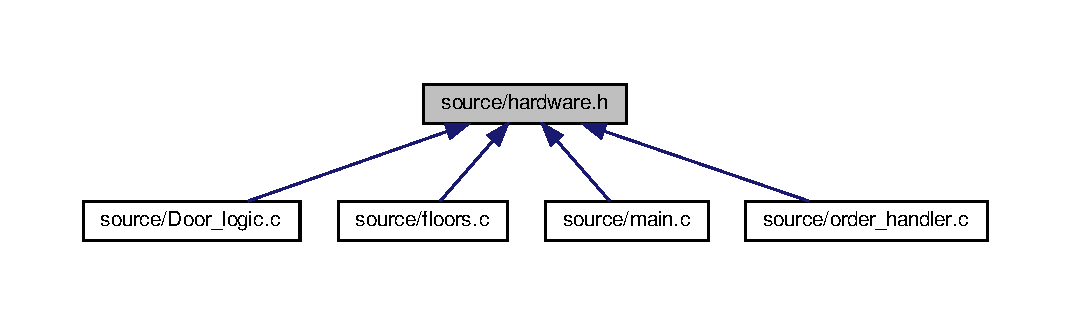
\includegraphics[width=350pt]{hardware_8h__dep__incl}
\end{center}
\end{figure}
\subsection*{Macros}
\begin{DoxyCompactItemize}
\item 
\mbox{\Hypertarget{hardware_8h_ae9e42615eade15633bd8c03b7a271a00}\label{hardware_8h_ae9e42615eade15633bd8c03b7a271a00}} 
\#define {\bfseries H\+A\+R\+D\+W\+A\+R\+E\+\_\+\+N\+U\+M\+B\+E\+R\+\_\+\+O\+F\+\_\+\+F\+L\+O\+O\+RS}~4
\end{DoxyCompactItemize}
\subsection*{Enumerations}
\begin{DoxyCompactItemize}
\item 
\mbox{\Hypertarget{hardware_8h_a2167c399a24df296afc432bcb88228af}\label{hardware_8h_a2167c399a24df296afc432bcb88228af}} 
enum \hyperlink{hardware_8h_a2167c399a24df296afc432bcb88228af}{Hardware\+Movement} \{ {\bfseries H\+A\+R\+D\+W\+A\+R\+E\+\_\+\+M\+O\+V\+E\+M\+E\+N\+T\+\_\+\+UP}, 
{\bfseries H\+A\+R\+D\+W\+A\+R\+E\+\_\+\+M\+O\+V\+E\+M\+E\+N\+T\+\_\+\+S\+T\+OP}, 
{\bfseries H\+A\+R\+D\+W\+A\+R\+E\+\_\+\+M\+O\+V\+E\+M\+E\+N\+T\+\_\+\+D\+O\+WN}
 \}\begin{DoxyCompactList}\small\item\em Movement type used in {\ttfamily hardware\+\_\+command\+\_\+movement}. \end{DoxyCompactList}
\item 
\mbox{\Hypertarget{hardware_8h_a796a8de8ce0ae769d7dbd3327a7bdbe7}\label{hardware_8h_a796a8de8ce0ae769d7dbd3327a7bdbe7}} 
enum \hyperlink{hardware_8h_a796a8de8ce0ae769d7dbd3327a7bdbe7}{Hardware\+Order} \{ {\bfseries H\+A\+R\+D\+W\+A\+R\+E\+\_\+\+O\+R\+D\+E\+R\+\_\+\+UP}, 
{\bfseries H\+A\+R\+D\+W\+A\+R\+E\+\_\+\+O\+R\+D\+E\+R\+\_\+\+I\+N\+S\+I\+DE}, 
{\bfseries H\+A\+R\+D\+W\+A\+R\+E\+\_\+\+O\+R\+D\+E\+R\+\_\+\+D\+O\+WN}
 \}\begin{DoxyCompactList}\small\item\em Order type used in {\ttfamily hardware\+\_\+read\+\_\+order} and in {\ttfamily hardware\+\_\+command\+\_\+order\+\_\+light}. \end{DoxyCompactList}
\end{DoxyCompactItemize}
\subsection*{Functions}
\begin{DoxyCompactItemize}
\item 
int \hyperlink{hardware_8h_a054b8fb8768311d46be58d6a4890d771}{hardware\+\_\+init} ()
\begin{DoxyCompactList}\small\item\em Initializes the elevator control hardware. Must be called once before other calls to the elevator hardware driver. \end{DoxyCompactList}\item 
void \hyperlink{hardware_8h_a01de081ef0510a111053c18cd31afa27}{hardware\+\_\+command\+\_\+movement} (\hyperlink{hardware_8h_a2167c399a24df296afc432bcb88228af}{Hardware\+Movement} movement)
\begin{DoxyCompactList}\small\item\em Commands the elevator to either move up or down, or commands it to halt. \end{DoxyCompactList}\item 
int \hyperlink{hardware_8h_a4a77b27c86675c00b513db3445966804}{hardware\+\_\+read\+\_\+stop\+\_\+signal} ()
\begin{DoxyCompactList}\small\item\em Polls the hardware for the current stop signal. \end{DoxyCompactList}\item 
int \hyperlink{hardware_8h_a459fe57a3ee4bc2a28e8a15b2ab14c2d}{hardware\+\_\+read\+\_\+obstruction\+\_\+signal} ()
\begin{DoxyCompactList}\small\item\em Polls the hardware for the current obstruction signal. \end{DoxyCompactList}\item 
int \hyperlink{hardware_8h_ab048489e6302bb5604aad753f2d7d501}{hardware\+\_\+read\+\_\+floor\+\_\+sensor} (int floor)
\begin{DoxyCompactList}\small\item\em Polls the floor sensor for the given {\ttfamily floor}. \end{DoxyCompactList}\item 
int \hyperlink{hardware_8h_a87917f3aa093fb46ca821a400d011ee8}{hardware\+\_\+read\+\_\+order} (int floor, \hyperlink{hardware_8h_a796a8de8ce0ae769d7dbd3327a7bdbe7}{Hardware\+Order} order\+\_\+type)
\begin{DoxyCompactList}\small\item\em Polls the hardware for the status of orders from floor {\ttfamily floor} of type {\ttfamily order\+\_\+type}. \end{DoxyCompactList}\item 
void \hyperlink{hardware_8h_a80d99ddaa8e7b58c9a88b60ea553c1b6}{hardware\+\_\+command\+\_\+door\+\_\+open} (int door\+\_\+open)
\begin{DoxyCompactList}\small\item\em Commands the hardware to open-\/ or close the elevator door. \end{DoxyCompactList}\item 
void \hyperlink{hardware_8h_a407a6ec035ba357de6aa0fbe55501d1e}{hardware\+\_\+command\+\_\+floor\+\_\+indicator\+\_\+on} (int floor)
\begin{DoxyCompactList}\small\item\em Commands the hardware to turn on the floor indicator for {\ttfamily floor}. All indicators all mutually exclusive; other indicator lights will turn off. \end{DoxyCompactList}\item 
void \hyperlink{hardware_8h_aa75b3ac17f72b25946414f48d0063a10}{hardware\+\_\+command\+\_\+stop\+\_\+light} (int on)
\begin{DoxyCompactList}\small\item\em Sets the light in the panel stop button. \end{DoxyCompactList}\item 
void \hyperlink{hardware_8h_aa9b33faa52f0ec5b614d3e7dc05be140}{hardware\+\_\+command\+\_\+order\+\_\+light} (int floor, \hyperlink{hardware_8h_a796a8de8ce0ae769d7dbd3327a7bdbe7}{Hardware\+Order} order\+\_\+type, int on)
\begin{DoxyCompactList}\small\item\em Sets the light in a button corresponding to an order of type {\ttfamily order\+\_\+type}, at floor {\ttfamily floor}. \end{DoxyCompactList}\end{DoxyCompactItemize}


\subsection{Detailed Description}
Driver for the elevator hardware. 

Neatly wraps up Martin Korsgaard\textquotesingle{}s spaghetti from 2006 ;)

Kolbjørn Austreng 

\subsection{Function Documentation}
\mbox{\Hypertarget{hardware_8h_a80d99ddaa8e7b58c9a88b60ea553c1b6}\label{hardware_8h_a80d99ddaa8e7b58c9a88b60ea553c1b6}} 
\index{hardware.\+h@{hardware.\+h}!hardware\+\_\+command\+\_\+door\+\_\+open@{hardware\+\_\+command\+\_\+door\+\_\+open}}
\index{hardware\+\_\+command\+\_\+door\+\_\+open@{hardware\+\_\+command\+\_\+door\+\_\+open}!hardware.\+h@{hardware.\+h}}
\subsubsection{\texorpdfstring{hardware\+\_\+command\+\_\+door\+\_\+open()}{hardware\_command\_door\_open()}}
{\footnotesize\ttfamily void hardware\+\_\+command\+\_\+door\+\_\+open (\begin{DoxyParamCaption}\item[{int}]{door\+\_\+open }\end{DoxyParamCaption})}



Commands the hardware to open-\/ or close the elevator door. 


\begin{DoxyParams}{Parameters}
{\em door\+\_\+open} & A truthy value (non-\/zero) to open the door; 0 to close. \\
\hline
\end{DoxyParams}
\mbox{\Hypertarget{hardware_8h_a407a6ec035ba357de6aa0fbe55501d1e}\label{hardware_8h_a407a6ec035ba357de6aa0fbe55501d1e}} 
\index{hardware.\+h@{hardware.\+h}!hardware\+\_\+command\+\_\+floor\+\_\+indicator\+\_\+on@{hardware\+\_\+command\+\_\+floor\+\_\+indicator\+\_\+on}}
\index{hardware\+\_\+command\+\_\+floor\+\_\+indicator\+\_\+on@{hardware\+\_\+command\+\_\+floor\+\_\+indicator\+\_\+on}!hardware.\+h@{hardware.\+h}}
\subsubsection{\texorpdfstring{hardware\+\_\+command\+\_\+floor\+\_\+indicator\+\_\+on()}{hardware\_command\_floor\_indicator\_on()}}
{\footnotesize\ttfamily void hardware\+\_\+command\+\_\+floor\+\_\+indicator\+\_\+on (\begin{DoxyParamCaption}\item[{int}]{floor }\end{DoxyParamCaption})}



Commands the hardware to turn on the floor indicator for {\ttfamily floor}. All indicators all mutually exclusive; other indicator lights will turn off. 


\begin{DoxyParams}{Parameters}
{\em floor} & Floor to turn on the indicator for.\\
\hline
\end{DoxyParams}
\begin{DoxyWarning}{Warning}
Owing to peculiarities in the hardware construction, there will always be one indicator active. 
\end{DoxyWarning}
\mbox{\Hypertarget{hardware_8h_a01de081ef0510a111053c18cd31afa27}\label{hardware_8h_a01de081ef0510a111053c18cd31afa27}} 
\index{hardware.\+h@{hardware.\+h}!hardware\+\_\+command\+\_\+movement@{hardware\+\_\+command\+\_\+movement}}
\index{hardware\+\_\+command\+\_\+movement@{hardware\+\_\+command\+\_\+movement}!hardware.\+h@{hardware.\+h}}
\subsubsection{\texorpdfstring{hardware\+\_\+command\+\_\+movement()}{hardware\_command\_movement()}}
{\footnotesize\ttfamily void hardware\+\_\+command\+\_\+movement (\begin{DoxyParamCaption}\item[{\hyperlink{hardware_8h_a2167c399a24df296afc432bcb88228af}{Hardware\+Movement}}]{movement }\end{DoxyParamCaption})}



Commands the elevator to either move up or down, or commands it to halt. 


\begin{DoxyParams}{Parameters}
{\em movement} & Commanded movement. \\
\hline
\end{DoxyParams}
\mbox{\Hypertarget{hardware_8h_aa9b33faa52f0ec5b614d3e7dc05be140}\label{hardware_8h_aa9b33faa52f0ec5b614d3e7dc05be140}} 
\index{hardware.\+h@{hardware.\+h}!hardware\+\_\+command\+\_\+order\+\_\+light@{hardware\+\_\+command\+\_\+order\+\_\+light}}
\index{hardware\+\_\+command\+\_\+order\+\_\+light@{hardware\+\_\+command\+\_\+order\+\_\+light}!hardware.\+h@{hardware.\+h}}
\subsubsection{\texorpdfstring{hardware\+\_\+command\+\_\+order\+\_\+light()}{hardware\_command\_order\_light()}}
{\footnotesize\ttfamily void hardware\+\_\+command\+\_\+order\+\_\+light (\begin{DoxyParamCaption}\item[{int}]{floor,  }\item[{\hyperlink{hardware_8h_a796a8de8ce0ae769d7dbd3327a7bdbe7}{Hardware\+Order}}]{order\+\_\+type,  }\item[{int}]{on }\end{DoxyParamCaption})}



Sets the light in a button corresponding to an order of type {\ttfamily order\+\_\+type}, at floor {\ttfamily floor}. 


\begin{DoxyParams}{Parameters}
{\em floor} & The floor of the order indicator. \\
\hline
{\em order\+\_\+type} & The type of order. \\
\hline
{\em on} & A truthy value (non-\/zero) to turn the light on; 0 to turn it off. \\
\hline
\end{DoxyParams}
\mbox{\Hypertarget{hardware_8h_aa75b3ac17f72b25946414f48d0063a10}\label{hardware_8h_aa75b3ac17f72b25946414f48d0063a10}} 
\index{hardware.\+h@{hardware.\+h}!hardware\+\_\+command\+\_\+stop\+\_\+light@{hardware\+\_\+command\+\_\+stop\+\_\+light}}
\index{hardware\+\_\+command\+\_\+stop\+\_\+light@{hardware\+\_\+command\+\_\+stop\+\_\+light}!hardware.\+h@{hardware.\+h}}
\subsubsection{\texorpdfstring{hardware\+\_\+command\+\_\+stop\+\_\+light()}{hardware\_command\_stop\_light()}}
{\footnotesize\ttfamily void hardware\+\_\+command\+\_\+stop\+\_\+light (\begin{DoxyParamCaption}\item[{int}]{on }\end{DoxyParamCaption})}



Sets the light in the panel stop button. 


\begin{DoxyParams}{Parameters}
{\em on} & A truthy value (non-\/zero) to turn the light on; 0 to turn it off. \\
\hline
\end{DoxyParams}
\mbox{\Hypertarget{hardware_8h_a054b8fb8768311d46be58d6a4890d771}\label{hardware_8h_a054b8fb8768311d46be58d6a4890d771}} 
\index{hardware.\+h@{hardware.\+h}!hardware\+\_\+init@{hardware\+\_\+init}}
\index{hardware\+\_\+init@{hardware\+\_\+init}!hardware.\+h@{hardware.\+h}}
\subsubsection{\texorpdfstring{hardware\+\_\+init()}{hardware\_init()}}
{\footnotesize\ttfamily int hardware\+\_\+init (\begin{DoxyParamCaption}{ }\end{DoxyParamCaption})}



Initializes the elevator control hardware. Must be called once before other calls to the elevator hardware driver. 

\begin{DoxyReturn}{Returns}
0 on success. Non-\/zero for failure. 
\end{DoxyReturn}
\mbox{\Hypertarget{hardware_8h_ab048489e6302bb5604aad753f2d7d501}\label{hardware_8h_ab048489e6302bb5604aad753f2d7d501}} 
\index{hardware.\+h@{hardware.\+h}!hardware\+\_\+read\+\_\+floor\+\_\+sensor@{hardware\+\_\+read\+\_\+floor\+\_\+sensor}}
\index{hardware\+\_\+read\+\_\+floor\+\_\+sensor@{hardware\+\_\+read\+\_\+floor\+\_\+sensor}!hardware.\+h@{hardware.\+h}}
\subsubsection{\texorpdfstring{hardware\+\_\+read\+\_\+floor\+\_\+sensor()}{hardware\_read\_floor\_sensor()}}
{\footnotesize\ttfamily int hardware\+\_\+read\+\_\+floor\+\_\+sensor (\begin{DoxyParamCaption}\item[{int}]{floor }\end{DoxyParamCaption})}



Polls the floor sensor for the given {\ttfamily floor}. 


\begin{DoxyParams}{Parameters}
{\em floor} & Inquired floor.\\
\hline
\end{DoxyParams}
\begin{DoxyReturn}{Returns}
1 if the elevator is at {\ttfamily floor}, otherwise 0; 
\end{DoxyReturn}
\mbox{\Hypertarget{hardware_8h_a459fe57a3ee4bc2a28e8a15b2ab14c2d}\label{hardware_8h_a459fe57a3ee4bc2a28e8a15b2ab14c2d}} 
\index{hardware.\+h@{hardware.\+h}!hardware\+\_\+read\+\_\+obstruction\+\_\+signal@{hardware\+\_\+read\+\_\+obstruction\+\_\+signal}}
\index{hardware\+\_\+read\+\_\+obstruction\+\_\+signal@{hardware\+\_\+read\+\_\+obstruction\+\_\+signal}!hardware.\+h@{hardware.\+h}}
\subsubsection{\texorpdfstring{hardware\+\_\+read\+\_\+obstruction\+\_\+signal()}{hardware\_read\_obstruction\_signal()}}
{\footnotesize\ttfamily int hardware\+\_\+read\+\_\+obstruction\+\_\+signal (\begin{DoxyParamCaption}{ }\end{DoxyParamCaption})}



Polls the hardware for the current obstruction signal. 

\begin{DoxyReturn}{Returns}
1 if the obstruction signal is high; 0 if it is low. 
\end{DoxyReturn}
\mbox{\Hypertarget{hardware_8h_a87917f3aa093fb46ca821a400d011ee8}\label{hardware_8h_a87917f3aa093fb46ca821a400d011ee8}} 
\index{hardware.\+h@{hardware.\+h}!hardware\+\_\+read\+\_\+order@{hardware\+\_\+read\+\_\+order}}
\index{hardware\+\_\+read\+\_\+order@{hardware\+\_\+read\+\_\+order}!hardware.\+h@{hardware.\+h}}
\subsubsection{\texorpdfstring{hardware\+\_\+read\+\_\+order()}{hardware\_read\_order()}}
{\footnotesize\ttfamily int hardware\+\_\+read\+\_\+order (\begin{DoxyParamCaption}\item[{int}]{floor,  }\item[{\hyperlink{hardware_8h_a796a8de8ce0ae769d7dbd3327a7bdbe7}{Hardware\+Order}}]{order\+\_\+type }\end{DoxyParamCaption})}



Polls the hardware for the status of orders from floor {\ttfamily floor} of type {\ttfamily order\+\_\+type}. 


\begin{DoxyParams}{Parameters}
{\em floor} & Inquired floor. \\
\hline
{\em order\+\_\+type} & \\
\hline
\end{DoxyParams}
\begin{DoxyReturn}{Returns}
1 if the combination of {\ttfamily floor} and {\ttfamily order\+\_\+type} is being requested, otherwise 0. 
\end{DoxyReturn}
\mbox{\Hypertarget{hardware_8h_a4a77b27c86675c00b513db3445966804}\label{hardware_8h_a4a77b27c86675c00b513db3445966804}} 
\index{hardware.\+h@{hardware.\+h}!hardware\+\_\+read\+\_\+stop\+\_\+signal@{hardware\+\_\+read\+\_\+stop\+\_\+signal}}
\index{hardware\+\_\+read\+\_\+stop\+\_\+signal@{hardware\+\_\+read\+\_\+stop\+\_\+signal}!hardware.\+h@{hardware.\+h}}
\subsubsection{\texorpdfstring{hardware\+\_\+read\+\_\+stop\+\_\+signal()}{hardware\_read\_stop\_signal()}}
{\footnotesize\ttfamily int hardware\+\_\+read\+\_\+stop\+\_\+signal (\begin{DoxyParamCaption}{ }\end{DoxyParamCaption})}



Polls the hardware for the current stop signal. 

\begin{DoxyReturn}{Returns}
1 if the stop signal is high; 0 if it is low. 
\end{DoxyReturn}

\hypertarget{order__handler_8h}{}\section{source/order\+\_\+handler.h File Reference}
\label{order__handler_8h}\index{source/order\+\_\+handler.\+h@{source/order\+\_\+handler.\+h}}


functions that record, change or delete orders and lights  


This graph shows which files directly or indirectly include this file\+:\nopagebreak
\begin{figure}[H]
\begin{center}
\leavevmode
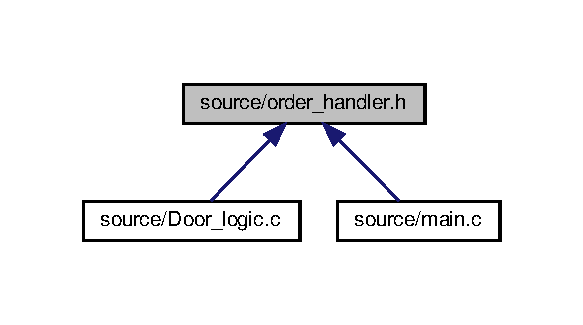
\includegraphics[width=280pt]{order__handler_8h__dep__incl}
\end{center}
\end{figure}
\subsection*{Functions}
\begin{DoxyCompactItemize}
\item 
void \hyperlink{order__handler_8h_a778303313380fee1b1b85c7276ccc565}{swap} (int $\ast$next\+\_\+order\+\_\+queue, int a, int b)
\begin{DoxyCompactList}\small\item\em A function made to swap a number at index a with a number at index b in an array. \end{DoxyCompactList}\item 
void \hyperlink{order__handler_8h_ab332e70ab2804ea51f6785d03abc46a8}{order\+\_\+record} (int $\ast$inside, int $\ast$up, int $\ast$down)
\begin{DoxyCompactList}\small\item\em A function made to record the orders that we give via the buttons and record $\ast$them in the corresponding array. \end{DoxyCompactList}\item 
void \hyperlink{order__handler_8h_a159acf8c0e75ec66c6e2d8f41bbb3df3}{order\+\_\+delete} (int $\ast$inside, int $\ast$up, int $\ast$down, int $\ast$next)
\begin{DoxyCompactList}\small\item\em A function made to delete all the orders from the arrays. Used with the stop button. \end{DoxyCompactList}\item 
void \hyperlink{order__handler_8h_a010a11a17a76600fcee792e16f64806e}{update\+\_\+lights\+\_\+and\+\_\+orders} (int floor, int $\ast$inside, int $\ast$up, int $\ast$down)
\begin{DoxyCompactList}\small\item\em A function made to turn of the lights and orders when we arrive at a corresponding floor. \end{DoxyCompactList}\item 
void \hyperlink{order__handler_8h_a007a8d621bc967016c1621937c095e5f}{update\+\_\+queue} (int $\ast$queue, int current\+\_\+floor)
\begin{DoxyCompactList}\small\item\em A function made to delete the current\+\_\+floor from the list of next orders, so the elevator doesn\textquotesingle{}t go to the same floor twice. It sets the first number to 0, then it shifts all number except the first one spot to the left. \end{DoxyCompactList}\item 
void \hyperlink{order__handler_8h_a8b444e8acd4d9949d10d7679256ac105}{set\+\_\+order\+\_\+lights} (int i)
\begin{DoxyCompactList}\small\item\em A function made to set all order lights when the corresponding button is pushed. If i is one it will cycle through all button and lights the button if it is pushed. If i is 0 (used with the stop button) all the lights will be set low. \end{DoxyCompactList}\item 
void \hyperlink{order__handler_8h_acf5362396e06c352829f23d221d08059}{order\+\_\+handler} (int $\ast$inside, int $\ast$up, int $\ast$down, int last\+\_\+direction, int $\ast$next\+\_\+order\+\_\+queue, int current\+\_\+floor, int state)
\begin{DoxyCompactList}\small\item\em A function that decides the priority of the orders. It useds the following steps\+: \end{DoxyCompactList}\end{DoxyCompactItemize}


\subsection{Detailed Description}
functions that record, change or delete orders and lights 



\subsection{Function Documentation}
\mbox{\Hypertarget{order__handler_8h_a159acf8c0e75ec66c6e2d8f41bbb3df3}\label{order__handler_8h_a159acf8c0e75ec66c6e2d8f41bbb3df3}} 
\index{order\+\_\+handler.\+h@{order\+\_\+handler.\+h}!order\+\_\+delete@{order\+\_\+delete}}
\index{order\+\_\+delete@{order\+\_\+delete}!order\+\_\+handler.\+h@{order\+\_\+handler.\+h}}
\subsubsection{\texorpdfstring{order\+\_\+delete()}{order\_delete()}}
{\footnotesize\ttfamily void order\+\_\+delete (\begin{DoxyParamCaption}\item[{int $\ast$}]{inside,  }\item[{int $\ast$}]{up,  }\item[{int $\ast$}]{down,  }\item[{int $\ast$}]{next }\end{DoxyParamCaption})}



A function made to delete all the orders from the arrays. Used with the stop button. 


\begin{DoxyParams}[1]{Parameters}
\mbox{\tt in,out}  & {\em inside} & The array of the orders from inside the elevator\\
\hline
\mbox{\tt in,out}  & {\em up} & The array of orders from outside the elevator going up\\
\hline
\mbox{\tt in,out}  & {\em down} & The array of orders from outside the elevator going down\\
\hline
\mbox{\tt in,out}  & {\em next} & The array that contains the next orders \\
\hline
\end{DoxyParams}


Definition at line 42 of file order\+\_\+handler.\+c.

\mbox{\Hypertarget{order__handler_8h_acf5362396e06c352829f23d221d08059}\label{order__handler_8h_acf5362396e06c352829f23d221d08059}} 
\index{order\+\_\+handler.\+h@{order\+\_\+handler.\+h}!order\+\_\+handler@{order\+\_\+handler}}
\index{order\+\_\+handler@{order\+\_\+handler}!order\+\_\+handler.\+h@{order\+\_\+handler.\+h}}
\subsubsection{\texorpdfstring{order\+\_\+handler()}{order\_handler()}}
{\footnotesize\ttfamily void order\+\_\+handler (\begin{DoxyParamCaption}\item[{int $\ast$}]{inside,  }\item[{int $\ast$}]{up,  }\item[{int $\ast$}]{down,  }\item[{int}]{last\+\_\+direction,  }\item[{int $\ast$}]{next\+\_\+order\+\_\+queue,  }\item[{int}]{current\+\_\+floor,  }\item[{int}]{state }\end{DoxyParamCaption})}



A function that decides the priority of the orders. It useds the following steps\+: 


\begin{DoxyItemize}
\item It checks if the direction is Up, Down or Stop. e.\+g. If the direction is up, it will only care about orders that are going up or from inside the elevator.
\item The first for-\/loop is used to cycle through all the orders and it will only proceed if there is an order which is the job of the if-\/statement.
\item The second for-\/loop is used to cycle through the next\+\_\+order\+\_\+queue to add the new orders, if an order to the same floor doesn\textquotesingle{}t already exit. Uesd to avoid duplicate orders.
\item The secret sauce is the third if statement. It prioritises the orders to make the execution more streamlined. e.\+g. if the 3. floor inside is pushed and the 2. floor up afterwards, and the elevator is below the 2. floor, it will take the 2. floor before the 3. it compares the first order in the next\+\_\+order\+\_\+queue and with the other orders at swaps them if it will come to another floor first.


\begin{DoxyParams}[1]{Parameters}
\mbox{\tt in}  & {\em current\+\_\+floor} & The floor we are currently at\\
\hline
\mbox{\tt in}  & {\em state} & The state we are currently in(Stationary\+\_\+f, Up ...)\\
\hline
\mbox{\tt in}  & {\em last\+\_\+direction} & The direction the elevator is travelling. 1= up, 2 = down, 0 = stop\\
\hline
\mbox{\tt in,out}  & {\em inside} & The array of the orders from inside the elevator\\
\hline
\mbox{\tt in,out}  & {\em up} & The array of the orders from outside the elevator going up\\
\hline
\mbox{\tt in,out}  & {\em down} & The array of the orders from outside the elevator going down\\
\hline
\mbox{\tt in,out}  & {\em next\+\_\+order\+\_\+queue} & The array that contains the next orders \\
\hline
\end{DoxyParams}

\end{DoxyItemize}

Definition at line 130 of file order\+\_\+handler.\+c.

\mbox{\Hypertarget{order__handler_8h_ab332e70ab2804ea51f6785d03abc46a8}\label{order__handler_8h_ab332e70ab2804ea51f6785d03abc46a8}} 
\index{order\+\_\+handler.\+h@{order\+\_\+handler.\+h}!order\+\_\+record@{order\+\_\+record}}
\index{order\+\_\+record@{order\+\_\+record}!order\+\_\+handler.\+h@{order\+\_\+handler.\+h}}
\subsubsection{\texorpdfstring{order\+\_\+record()}{order\_record()}}
{\footnotesize\ttfamily void order\+\_\+record (\begin{DoxyParamCaption}\item[{int $\ast$}]{inside,  }\item[{int $\ast$}]{up,  }\item[{int $\ast$}]{down }\end{DoxyParamCaption})}



A function made to record the orders that we give via the buttons and record $\ast$them in the corresponding array. 


\begin{DoxyParams}[1]{Parameters}
\mbox{\tt in,out}  & {\em inside} & The array of the orders from inside the elevator\\
\hline
\mbox{\tt in,out}  & {\em up} & The array of the orders from outside the elevator going up\\
\hline
\mbox{\tt in,out}  & {\em down} & The array of the orders from outside the elevator going down \\
\hline
\end{DoxyParams}


Definition at line 11 of file order\+\_\+handler.\+c.

\mbox{\Hypertarget{order__handler_8h_a8b444e8acd4d9949d10d7679256ac105}\label{order__handler_8h_a8b444e8acd4d9949d10d7679256ac105}} 
\index{order\+\_\+handler.\+h@{order\+\_\+handler.\+h}!set\+\_\+order\+\_\+lights@{set\+\_\+order\+\_\+lights}}
\index{set\+\_\+order\+\_\+lights@{set\+\_\+order\+\_\+lights}!order\+\_\+handler.\+h@{order\+\_\+handler.\+h}}
\subsubsection{\texorpdfstring{set\+\_\+order\+\_\+lights()}{set\_order\_lights()}}
{\footnotesize\ttfamily void set\+\_\+order\+\_\+lights (\begin{DoxyParamCaption}\item[{int}]{i }\end{DoxyParamCaption})}



A function made to set all order lights when the corresponding button is pushed. If i is one it will cycle through all button and lights the button if it is pushed. If i is 0 (used with the stop button) all the lights will be set low. 


\begin{DoxyParams}[1]{Parameters}
\mbox{\tt in}  & {\em i} & This int decides if the lights should be set as normal(1) or reset at turned off(0) \\
\hline
\end{DoxyParams}


Definition at line 57 of file order\+\_\+handler.\+c.

\mbox{\Hypertarget{order__handler_8h_a778303313380fee1b1b85c7276ccc565}\label{order__handler_8h_a778303313380fee1b1b85c7276ccc565}} 
\index{order\+\_\+handler.\+h@{order\+\_\+handler.\+h}!swap@{swap}}
\index{swap@{swap}!order\+\_\+handler.\+h@{order\+\_\+handler.\+h}}
\subsubsection{\texorpdfstring{swap()}{swap()}}
{\footnotesize\ttfamily void swap (\begin{DoxyParamCaption}\item[{int $\ast$}]{next\+\_\+order\+\_\+queue,  }\item[{int}]{a,  }\item[{int}]{b }\end{DoxyParamCaption})}



A function made to swap a number at index a with a number at index b in an array. 


\begin{DoxyParams}[1]{Parameters}
\mbox{\tt in,out}  & {\em next\+\_\+order\+\_\+queue} & The queue of orders that we want to change\\
\hline
\mbox{\tt in}  & {\em a} & An int that indicate the spot of the number we want to change\\
\hline
\mbox{\tt in}  & {\em b} & An int that indicate the spot of the number we want to change$>$ \\
\hline
\end{DoxyParams}


Definition at line 104 of file order\+\_\+handler.\+c.

\mbox{\Hypertarget{order__handler_8h_a010a11a17a76600fcee792e16f64806e}\label{order__handler_8h_a010a11a17a76600fcee792e16f64806e}} 
\index{order\+\_\+handler.\+h@{order\+\_\+handler.\+h}!update\+\_\+lights\+\_\+and\+\_\+orders@{update\+\_\+lights\+\_\+and\+\_\+orders}}
\index{update\+\_\+lights\+\_\+and\+\_\+orders@{update\+\_\+lights\+\_\+and\+\_\+orders}!order\+\_\+handler.\+h@{order\+\_\+handler.\+h}}
\subsubsection{\texorpdfstring{update\+\_\+lights\+\_\+and\+\_\+orders()}{update\_lights\_and\_orders()}}
{\footnotesize\ttfamily void update\+\_\+lights\+\_\+and\+\_\+orders (\begin{DoxyParamCaption}\item[{int}]{floor,  }\item[{int $\ast$}]{inside,  }\item[{int $\ast$}]{up,  }\item[{int $\ast$}]{down }\end{DoxyParamCaption})}



A function made to turn of the lights and orders when we arrive at a corresponding floor. 


\begin{DoxyParams}[1]{Parameters}
\mbox{\tt in}  & {\em floor} & The floor we are currently at\\
\hline
\mbox{\tt in,out}  & {\em inside} & The array of the orders from inside the elevator\\
\hline
\mbox{\tt in,out}  & {\em up} & The array of the orders from outside the elevator going up\\
\hline
\mbox{\tt in,out}  & {\em down} & The array of the orders from outside the elevator going down \\
\hline
\end{DoxyParams}


Definition at line 89 of file order\+\_\+handler.\+c.

\mbox{\Hypertarget{order__handler_8h_a007a8d621bc967016c1621937c095e5f}\label{order__handler_8h_a007a8d621bc967016c1621937c095e5f}} 
\index{order\+\_\+handler.\+h@{order\+\_\+handler.\+h}!update\+\_\+queue@{update\+\_\+queue}}
\index{update\+\_\+queue@{update\+\_\+queue}!order\+\_\+handler.\+h@{order\+\_\+handler.\+h}}
\subsubsection{\texorpdfstring{update\+\_\+queue()}{update\_queue()}}
{\footnotesize\ttfamily void update\+\_\+queue (\begin{DoxyParamCaption}\item[{int $\ast$}]{queue,  }\item[{int}]{current\+\_\+floor }\end{DoxyParamCaption})}



A function made to delete the current\+\_\+floor from the list of next orders, so the elevator doesn\textquotesingle{}t go to the same floor twice. It sets the first number to 0, then it shifts all number except the first one spot to the left. 


\begin{DoxyParams}[1]{Parameters}
\mbox{\tt in}  & {\em current\+\_\+floor} & The floor we are currently at\\
\hline
\mbox{\tt in,out}  & {\em queue} & The array that contains the next orders \\
\hline
\end{DoxyParams}


Definition at line 115 of file order\+\_\+handler.\+c.


\hypertarget{Timer_8h}{}\section{source/\+Timer.h File Reference}
\label{Timer_8h}\index{source/\+Timer.\+h@{source/\+Timer.\+h}}
This graph shows which files directly or indirectly include this file\+:
\nopagebreak
\begin{figure}[H]
\begin{center}
\leavevmode
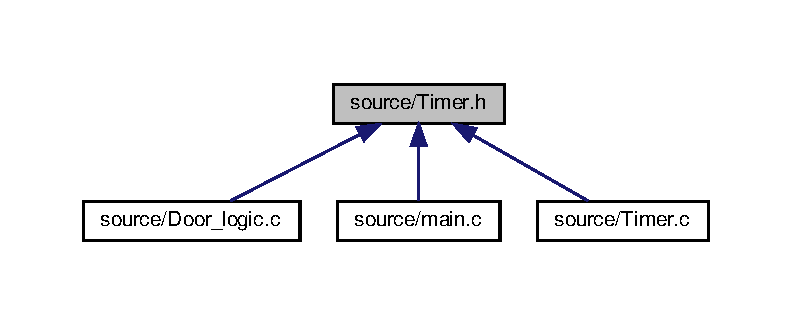
\includegraphics[width=350pt]{Timer_8h__dep__incl}
\end{center}
\end{figure}
\subsection*{Functions}
\begin{DoxyCompactItemize}
\item 
\mbox{\Hypertarget{Timer_8h_aaedac22c55880495505bf375e0e132c1}\label{Timer_8h_aaedac22c55880495505bf375e0e132c1}} 
void \hyperlink{Timer_8h_aaedac22c55880495505bf375e0e132c1}{start\+\_\+timer} ()
\begin{DoxyCompactList}\small\item\em Initializes a time with a set value since a given date (1/1 -\/ 1970) \end{DoxyCompactList}\item 
\mbox{\Hypertarget{Timer_8h_a703d741dc9d367d9e2ca654e3c8a34be}\label{Timer_8h_a703d741dc9d367d9e2ca654e3c8a34be}} 
int {\bfseries read\+\_\+timer} (int seconds)
\end{DoxyCompactItemize}


\subsection{Detailed Description}
brief Timer for the elevator 
%--- End generated contents ---

% Index
\backmatter
\newpage
\phantomsection
\clearemptydoublepage
\addcontentsline{toc}{chapter}{Index}
\printindex

\end{document}
